\documentclass{article}

% if you need to pass options to natbib, use, e.g.:
%     \PassOptionsToPackage{numbers, compress}{natbib}
% before loading neurips_2024


% ready for submission
% \usepackage{neurips_2024}


% to compile a preprint version, e.g., for submission to arXiv, add add the
% [preprint] option:
     \usepackage[preprint]{neurips_2024}


% to compile a camera-ready version, add the [final] option, e.g.:
%     \usepackage[final]{neurips_2024}


% to avoid loading the natbib package, add option nonatbib:
%    \usepackage[nonatbib]{neurips_2024}


\usepackage[utf8]{inputenc} % allow utf-8 input
\usepackage[T1]{fontenc}    % use 8-bit T1 fonts
\usepackage{hyperref}       % hyperlinks
\usepackage{url}            % simple URL typesetting
\usepackage{booktabs}       % professional-quality tables
\usepackage{amsfonts}       % blackboard math symbols
\usepackage{nicefrac}       % compact symbols for 1/2, etc.
\usepackage{microtype}      % microtypography
\usepackage{xcolor}         % colors
\usepackage{amsmath}
\usepackage{natbib}
\usepackage{graphicx}  % For including graphics
\usepackage{float}     % To control figure placement
\usepackage{geometry}
\usepackage{array}
\usepackage{multirow}
\usepackage{graphicx}
\usepackage{subcaption}



\title{Deep Learning 1 - Homework 3}


% The \author macro works with any number of authors. There are two commands
% used to separate the names and addresses of multiple authors: \And and \AND.
%
% Using \And between authors leaves it to LaTeX to determine where to break the
% lines. Using \AND forces a line break at that point. So, if LaTeX puts 3 of 4
% authors names on the first line, and the last on the second line, try using
% \AND instead of \And before the third author name.


\author{%
  Pedro M.P.~Curvo \\
  MSc Artificial Intelligence\\
  University of Amsterdam\\
  \texttt{pedro.pombeiro.curvo@student.uva.nl} \\
  % examples of more authors
  % \And
  % Coauthor \\
  % Affiliation \\
  % Address \\
  % \texttt{email} \\
  % \AND
  % Coauthor \\
  % Affiliation \\
  % Address \\
  % \texttt{email} \\
  % \And
  % Coauthor \\
  % Affiliation \\
  % Address \\
  % \texttt{email} \\
  % \And
  % Coauthor \\
  % Affiliation \\
  % Address \\
  % \texttt{email} \\
}


\begin{document}


\maketitle


% \begin{abstract}
%   The abstract paragraph should be indented \nicefrac{1}{2}~inch (3~picas) on
%   both the left- and right-hand margins. Use 10~point type, with a vertical
%   spacing (leading) of 11~points.  The word \textbf{Abstract} must be centered,
%   bold, and in point size 12. Two line spaces precede the abstract. The abstract
%   must be limited to one paragraph.
% \end{abstract}


\section*{Part 1}

\subsection*{1.1}

To sample an image using the decoder $f_{\theta}$ from the generative model described in this section, we first
need to sample a latent vector $z$ from the prior distribution $p(z)$. In this case, the prior distribution is a
standard multivariate Gaussian distribution, so we can sample $z$ from a standard normal distribution, i.e., $z \sim \mathcal{N}(0, I_D)$.
Then, we need to compute the pixel probabilities using the decoder $f_{\theta}$. For this, we pass
the sampled latent vector $z$ through the decoder $f_{\theta}$, which is a neural network parameterized by $\theta$.
This will map the latent vector $z$ to the probabilities of the Categorical distribution for each pixel $x_m$ in the image.
$f_{\theta}(z) \rightarrow (p_1, p_2, ..., p_k)^M$. 
Here: $p_m = (p_{m1}, p_{m2}, ..., p_{mk})$ are the event probabilities for pixel $m$ being in one of the $k$ categories.
$M$ is the number of pixels in the image. 
The, we can sample pixel values $x_n$ for each pixel $m$ by sampling from the Categorical distribution $Cat(x_m | f_{\theta}(z)_m)$.
Where, $x_m \sim Cat(p_m)$. This will generate the image by sampling each pixel value independently based on the
probabilities computed by the decoder. 
Finally we combine the pixel values $x_m$ to from the image $x_n$. 

\subsection*{1.2}

Monte Carlo integration with samples from $p(z_n)$ can be used to approximate the expectation of the log-likelihood. 
However, is inefficient for training VAE models because it requires a large number of samples to accurately estimate the
log-likelihood. This problem appears because the dimensionality of the latent space $z$ affects the number of samples
needed to cover the entire latent space adequately. As the dimensionality of the latent space increases, the space
becomes sparser, and more samples are needed to cover the space to capture the posterior distribution $p(z|x)$, which
is often highly concentrated in certain regions of the latent space (as shown by the blue contours in Figure 2).

This results in a exponentially increasing number of samples needed to accurately estimate the log-likelihood, 
that is, $L \rightarrow \infty$ as $D \rightarrow \infty$. This makes Monte Carlo integration impractical for high-dimensional
latent spaces due to the computational cost of sampling a large number of points to estimate the log-likelihood accurately.
Therefore, other methods are used to estimate the log-likelihood in VAE models. 

\subsection*{1.3}

From Equation 10, we have:

\begin{align*}
    \log p(x_n) - KL(q_{\theta}(z_n|x_n) || p(z_n|x_n)) &= \mathbb{E}_{q_{\theta}(z_n|x_n)}[\log p(x_n|z_n)] - KL(q_{\theta}(z_n|x_n) || p(z_n)) \\
\end{align*}

Rearranging the equation we get: 

\begin{align*}
    \log p(x_n) &= \mathbb{E}_{q_{\theta}(z_n|x_n)}[\log p(x_n|z_n)] - KL(q_{\theta}(z_n|x_n) || p(z_n)) + KL(q_{\theta}(z_n|x_n) || p(z_n|x_n)) \\
\end{align*}

Now, we know the KL divergence is always non-negative, since it is a measure of the difference between two distributions by
measuring how much one probability distribution diverges from a second, expected probability distribution. It is zero if and only if the two distributions are the same.
Mathematically, we have that: 

\begin{align*}
    KL(q_{\theta}(z_n|x_n) || p(z_n)) &\geq 0 \\
    KL(q_{\theta}(z_n|x_n) || p(z_n|x_n)) &\geq 0 \\
\end{align*}

With this we have that: 

\begin{align*}
  \log p(x_n) &= \mathbb{E}_{q_{\theta}(z_n|x_n)}[\log p(x_n|z_n)] - KL(q_{\theta}(z_n|x_n) || p(z_n)) + KL(q_{\theta}(z_n|x_n) || p(z_n|x_n)) \\
  &\geq \mathbb{E}_{q_{\theta}(z_n|x_n)}[\log p(x_n|z_n)] - KL(q_{\theta}(z_n|x_n) || p(z_n)) \\
\end{align*}

Therefore, the right-hand side of the equation $\mathbb{E}_{q_{\theta}(z_n|x_n)}[\log p(x_n|z_n)] - KL(q_{\theta}(z_n|x_n) || p(z_n))$ is
always less than or equal to the true log-likelihood $\log p(x_n)$. Hence, the right-hand side of the equation is a lower bound on the true log-likelihood.


\subsection*{1.4}

ELBO consists of two terms: 

\begin{align*}
    ELBO(x_n) &= \mathbb{E}_{q_{\theta}(z_n|x_n)}[\log p(x_n|z_n)] - KL(q_{\theta}(z_n|x_n) || p(z_n)) \\
\end{align*}

The first term, $\mathbb{E}_{q_{\theta}(z_n|x_n)}[\log p(x_n|z_n)]$, represents the expected log-likelihood of the data $x_n$ given the latent variable $z_n$.
However, this value stays the same regardless of how $q(z_n|x_n)$ is chosen.
The second term, $KL(q_{\theta}(z_n|x_n) || p(z_n))$, represents the KL divergence between the approximate posterior $q_{\theta}(z_n|x_n)$ and the prior $p(z_n)$.
As $q_{\theta}(z_n|x_n)$ approaches the true posterior $p(z_n|x_n)$, the KL divergence term decreases towards zero. This
is because the KL divergence is minimized when the two distributions are the same, $q(z_n|x_n) = p(z_n|x_n)$.
With that being said, as the KL divergence term decreases, the ELBO increases. becoming closer to the true log-likelihood $\log p(x_n)$.
Ideally, when $q(z_n|x_n) = p(z_n|x_n)$, the ELBO is equal to the true log-likelihood $\log p(x_n)$.

So: 

\begin{align*}
    \lim_{q_{\theta}(z_n|x_n) \rightarrow p(z_n|x_n)} ELBO(x_n) &= \lim_{q_{\theta}(z_n|x_n) \rightarrow p(z_n|x_n)} \mathbb{E}_{q_{\theta}(z_n|x_n)}[\log p(x_n|z_n)] - KL(q_{\theta}(z_n|x_n) || p(z_n)) \\
    &= \mathbb{E}_{p(z_n|x_n)}[\log p(x_n|z_n)] - \lim_{q_{\theta}(z_n|x_n) \rightarrow p(z_n|x_n)} KL(q_{\theta}(z_n|x_n) || p(z_n)) \\
    &= \mathbb{E}_{p(z_n|x_n)}[\log p(x_n|z_n)] - KL(p(z_n|x_n) || p(z_n)) \\
    &= \mathbb{E}_{p(z_n|x_n)}[\log p(x_n|z_n)] - 0 \\
    &= \mathbb{E}_{p(z_n|x_n)}[\log p(x_n|z_n)] \\
    &= \log p(x_n) \\
\end{align*}

And that is why the main goal of training a VAE is to maximize the ELBO, as it is a lower bound on the true log-likelihood $\log p(x_n)$.
And this corresponds to minimizing the KL divergence between the approximate posterior $q_{\theta}(z_n|x_n)$ and the prior $p(z_n)$.

\subsection*{1.5}

The names \textbf{reconstruction} loss and \textbf{regularization} loss are used because: 

\begin{itemize}
  \item \textbf{Reconstruction Loss}: The term $\mathbb{E}_{q_{\theta}(z_n|x_n)}[\log p(x_n|z_n)]$ is the expected log-likelihood
  of the data $x_n$ given the latent variable $z_n$. Hence, it is a measure of how well the model can reconstruct the
  observed data $x_n$ from the latent variable $z_n$. Meaning, it directly corresponds to the task of reconstructing the
  original input, being the main objective of the model. Therefore, it is called the \textbf{reconstruction} loss.

  \item\textbf{Regularization Loss:} The term $KL(q_{\theta}(z_n|x_n) || p(z_n))$ is the KL divergence and ensures
that the learned posterior distribution $q_{\theta}(z_n|x_n)$ is close to the prior distribution $p(z_n)$. This term
regularizes the model by preventing the posterior distribution from deviating too much from the prior distribution.
Therefore, it is called the \textbf{regularization} loss.
\end{itemize}

\subsection*{1.6}

When the prior distribution $p(z_n)$ is and variational posterior $q_{\theta}(z_n|x_n)$ are not Gaussian, the KL divergence
term $KL(q_{\theta}(z_n|x_n) || p(z_n))$ cannot be computed simply in closed form. To overcome this, we can use the
Monte Carlo approximation to estimate the regularization term. 

The regularization term in the VAE is the KL divergence between the variational distribution $q_{\theta}(z_n|x_n)$ and the prior distribution $p(z_n)$.
Mathematically, this term is defined as:

\begin{align*}
    D_{KL}(q_{\theta}(z_n|x_n) || p(z_n)) &= \mathbb{E}_{q_{\theta}(z_n|x_n)}[\log \frac{q_{\theta}(z_n|x_n)}{p(z_n)}] \\
\end{align*}

Assuming the closed-form expression for the KL divergence is intractable, we can use the Monte Carlo approximation to estimate the KL divergence.
First, we sample $L$ latent vectors $z_n^{(l)}$ from the variational distribution $q_{\theta}(z_n|x_n)$, where $l = 1, 2, ..., L$.
Then, we compute the log-ratio of the variational distribution and the prior distribution for each sample:

\begin{align*}
    \log \frac{q_{\theta}(z_n^{(l)}|x_n)}{p(z_n)} \\
\end{align*}

where $q_{\theta}(z_n^{(l)}|x_n)$ is the probability density of the variational distribution evaluated at the sample $z_n^{(l)}$.
Finally, we compute the Monte Carlo estimate of the KL divergence as:

\begin{align*}
    D_{KL}(q_{\theta}(z_n|x_n) || p(z_n)) &\approx \frac{1}{L} \sum_{l=1}^{L} \log \frac{q_{\theta}(z_n^{(l)}|x_n)}{p(z_n)} \\
\end{align*}

Then, we can use this approximation in the loss function:

\begin{align*}
    \mathbb{L}_{regularization,n} &\approx \frac{1}{L} \sum_{l=1}^{L} \log \frac{q_{\theta}(z_n^{(l)}|x_n)}{p(z_n)} \\
\end{align*}

This methods allows us to estimate the KL divergence term when the prior and variational posterior are not Gaussian. The more
samples we use, the more accurate the estimate will be, but it will also increase the computational cost of training the model.
This method can be used for any arbitrary prior and variational posterior distributions, as long as we can sample from the variational distribution
and compute the log-ratio of the two distributions.

It is also important to note the in this case the sampling is more efficient than the Monte Carlo integration for estimating the log-likelihood.
Sampling from $p(z_n)$ can lead to a more inefficient sampling because the prior may not capture the actual structure of the data, 
that is, many samples may be drawn from regions of $z_n$ that do not contribute to $p(x_n | z_n)$, leading to a poor estimate of the log-likelihood,
as seen in the image, where the prior distribution is a standard normal distribution. However, $p(z_n | x_n)$ is more concentrated
in specific regions of the latent space (the blue contours in the image).
However, by sampling from $q_{\theta}(z_n|x_n)$, we can sample from a distribution that is more likely to capture the structure of the data.
The variational distribution $q_{\theta}(z_n|x_n)$ is designed to be a good approximation of the true posterior $p(z_n|x_n)$,
Hence, samples drawn from $q_{\theta}(z_n|x_n)$ are more likely to be in regions of the latent space that contribute to the log-likelihood. 
In other words, the samples drawn from $q_{\theta}(z_n|x_n)$ are concentrated in areas where the posterior is high, which makes tgese
samples more useful. This lead to a more efficient Monte-Carlo integration because fewer samples are needed to estimate the
log-likelihood accurately.

\subsection*{1.7}

When we sample directly from a distribution $q_{\theta}(z_n|x_n)$ to estimate the expectation $\mathbb{E}_{q_{\theta}(z_n|x_n)}[\log p(x_n|z_n)]$,
the sampling part is non-differentiable with respect to the parameters $\theta$ of the model. This means that
the gradients with respect to the encoder parameters $\theta$ cannot be computed directly since the sampling operation does
not provide a smooth path for backpropagation. This is because the sampling operation introduces a discontinuity in the
computation graph, which makes it impossible to compute the gradients using standard backpropagation.

The reparameterization trick is a technique used to make the sampling operation differentiable with respect to the parameters $\theta$.
The trick involves reparameterizing the random variable $z_n$ as a deterministic function of the encoder outputs
$\mu_{\theta}(x_n)$ and $\sigma_{\theta}(x_n)$, and a noise variable $\epsilon$ sampled from a fixed distribution, such as a standard normal distribution,
i.e., $\epsilon \sim \mathcal{N}(0, I_D)$. This way the sample $z_n$ can be expressed as:

\begin{align*}
    z_n = \mu_{\theta}(x_n) + \sigma_{\theta}(x_n) \odot \epsilon \\
\end{align*}

With this, the sampling operation is now differentiable with respect to the parameters $\theta$ of the model. Allowing
us to compute the gradients of the loss function with respect to the parameters $\theta$ using backpropagation through the
encoder network. 

\subsection*{1.8}

\begin{table}[H]
    \centering
    \begin{tabular}{|c|}
    \hline
    \textbf{Test BPD} \\
    \hline
    1.912 \\
    \hline
    \end{tabular}
\end{table}

\begin{figure}[H]
    \centering
    \begin{minipage}{0.45\textwidth}
        \centering
        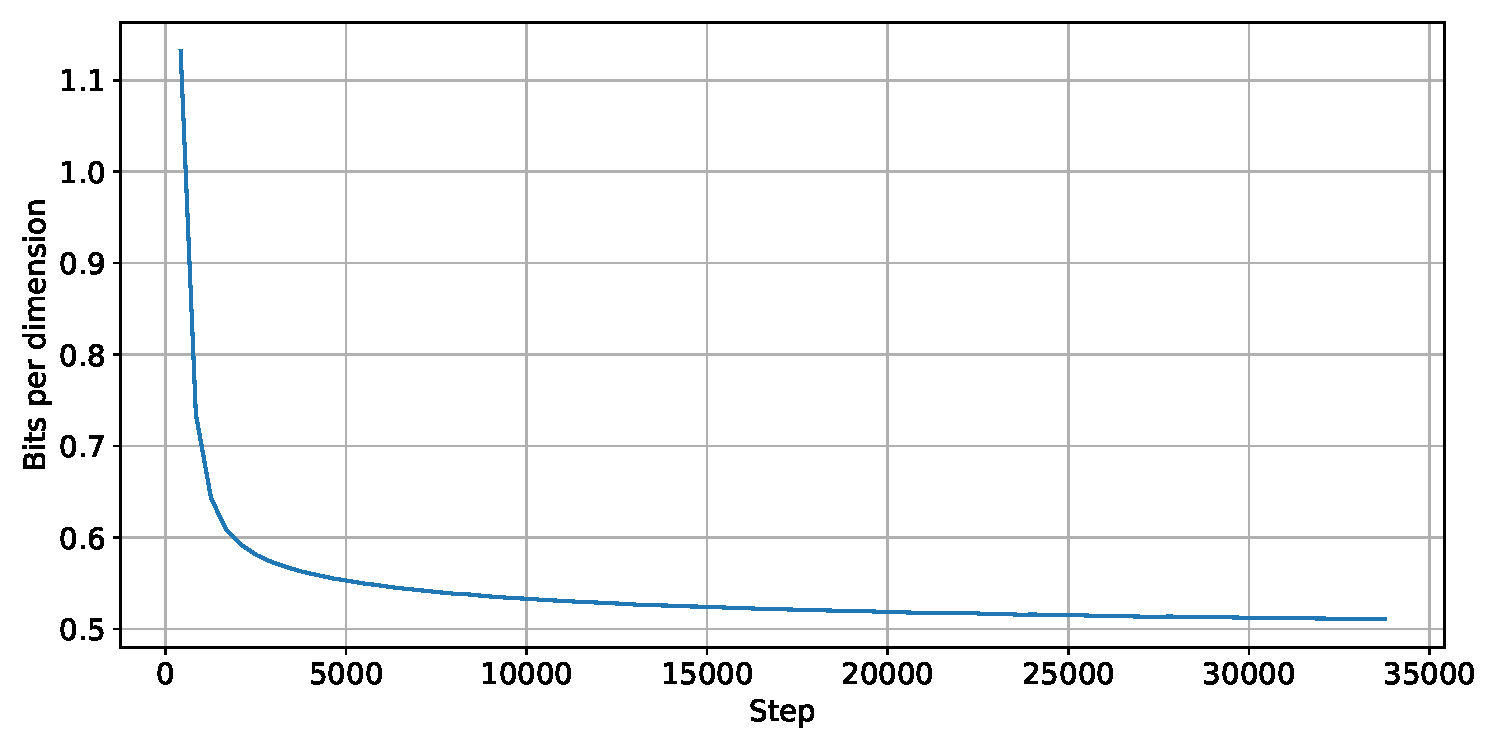
\includegraphics[width=\textwidth]{images/train_bpd.pdf}
        \caption{Train BPD}
        \label{fig:train_bpd}
    \end{minipage}
    \hfill
    \begin{minipage}{0.45\textwidth}
        \centering
        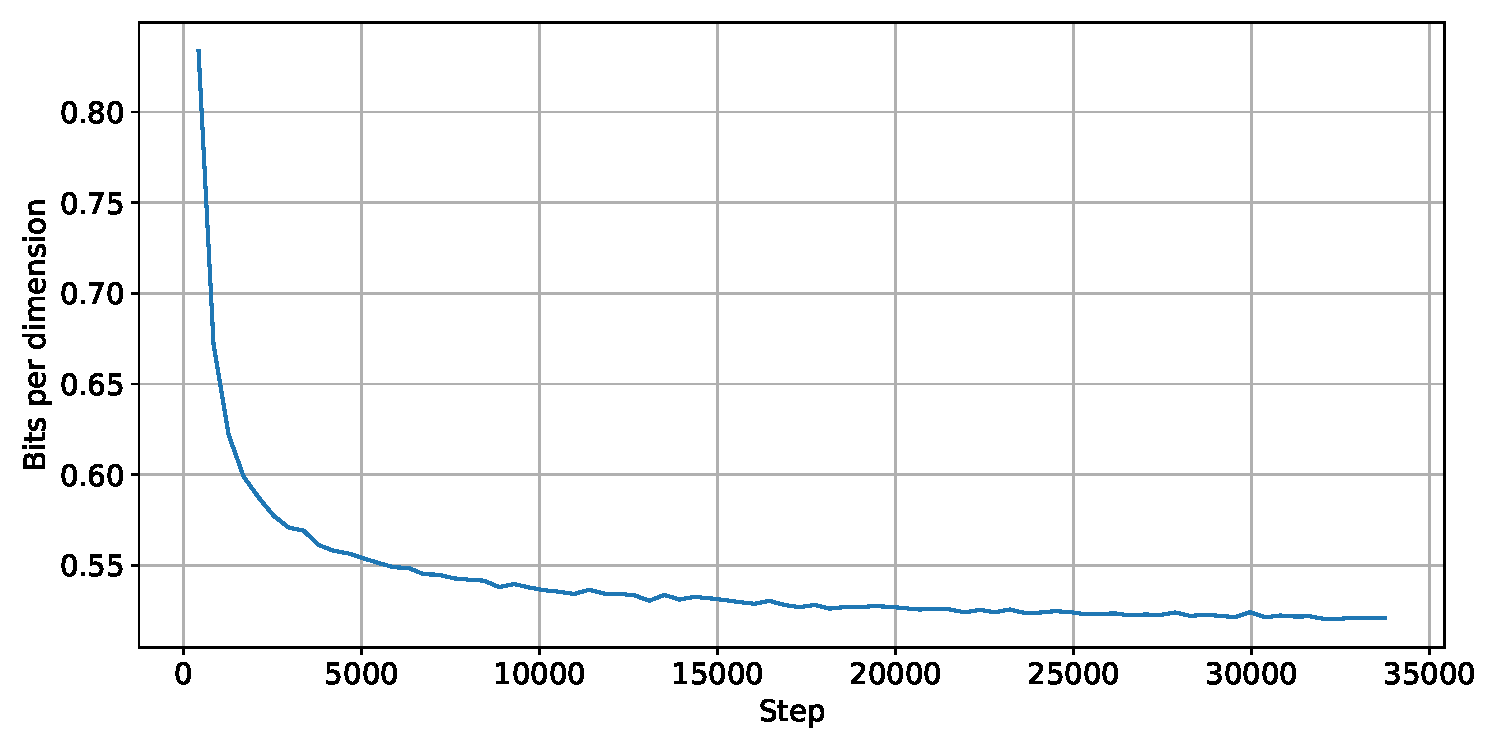
\includegraphics[width=\textwidth]{images/val_bpd.pdf}
        \caption{Validation BPD}
        \label{fig:val_bpd}
    \end{minipage}
    \caption{Train and Validation BPD for VAE with latent dim=20}
    \label{fig:vae_bpd}
\end{figure}

\subsection*{1.9}

\begin{figure}[H]
    \centering
    \begin{minipage}{0.3\textwidth}
        \centering
        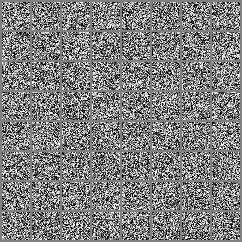
\includegraphics[width=\textwidth]{images/epoch_0_samples.png}
        \caption{Epoch 0}
        \label{fig:epoch_0}
    \end{minipage}
    \hfill
    \begin{minipage}{0.3\textwidth}
        \centering
        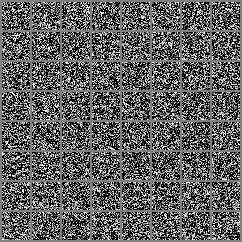
\includegraphics[width=\textwidth]{images/epoch_10_samples.png}
        \caption{Epoch 10}
        \label{fig:epoch_10}
    \end{minipage}
    \hfill
    \begin{minipage}{0.3\textwidth}
        \centering
        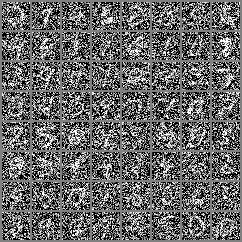
\includegraphics[width=\textwidth]{images/epoch_80_samples.png}
        \caption{Epoch 80}
        \label{fig:epoch_80}
    \end{minipage}
    \caption{Visualization of the VAE training progress at epochs 0, 10, and 80.}
    \label{fig:vae_epochs}
\end{figure}

By looking at the images generated by the VAE model before training, middle of training, and after training, we can see that
initially we only have noise in the images, as the model has not learned to generate meaningful images yet. As the model
trains, the images start to become more recognizable, and we start to see some numbers appearing in the images resembling
the digits in the MNIST dataset. At the end of training, I see that the images didn't improve much from the middle of training.
I believe this is the case, since the regularization loss keeps increasing. 

\subsection*{1.10}

% Manifold image 

% Manifold image 
\begin{figure}[H]
    \centering
    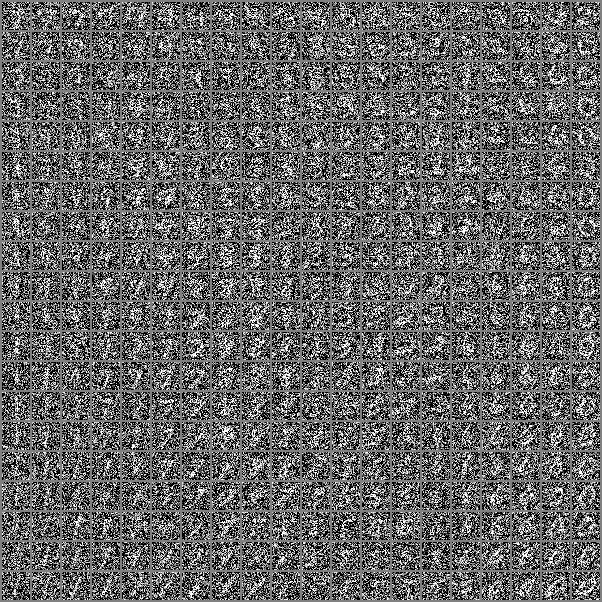
\includegraphics[width=0.8\textwidth]{images/vae_manifold.png}
    \caption{Visualization of the data manifold learned by the VAE. The manifold shows the reconstructed images from the
    2-dimensional latent space.}
    \label{fig:vae_manifold}
\end{figure}

In the image above, we observe that points in the latent space that correspond to similar digits form cluster, that is,
they are close and occupy a region of the plot. That way, the VAE encoded similar digits closer in the latent space.


\newpage
\section*{Part 2}

\subsection*{2.1}

% Table with arguments 
\begin{table}[h!]
    \centering
    \begin{tabular}{|c|c|c|c|c|c|c|}
    \hline
    \textbf{Argument} & \textbf{batch\_size} & \textbf{valid\_ratio} & \textbf{augmentations} & \textbf{pretrained} & \textbf{num\_epochs} & \textbf{train\_strats} \\
    \hline
    \textbf{Value} & 64 & 0.75 & False & True & 30 & ['standard'] \\
    \hline
    \textbf{Argument} & \textbf{visualise} & \textbf{epsilon\_fgsm} & \textbf{alpha\_fgsm} & \textbf{epsilon\_pgd} & \textbf{alpha\_pgd} & \textbf{num\_iter\_pgd} \\
    \hline
    \textbf{Value} & True & 0.1 & 0.5 & 0.01 & 2 & 10 \\
    \hline
    \end{tabular}
    \caption{Configuration used for a pretrained ResNet18 with and without FGSM attack}
\end{table}

\begin{table}[h!]
    \centering
    \begin{tabular}{|c|c|c|}
    \hline
    \textbf{Attack Test Type} & \textbf{Parameters} & \textbf{Test Accuracy} \\
    \hline
    Without & - & 0.93 \\
    \hline
    FGSM & Alpha: 0.5, Epsilon: 0.1 & 0.41 \\
    \hline
    PGD & Alpha: 2, Epsilon: 0.01, Num Iter: 10 & 0.4228 \\
    \hline
    \end{tabular}
    \caption{Testing results for \textbf{standard} training loss for different attacks using a \textbf{pretrained} ResNet18}
\end{table}



\begin{itemize}
    \item \textbf{i)} Adding a random perturbation of size $\epsilon$ does not target the specific vulnerability of the model,
    but rather adds noise to the input data. FGSM, on the other hand, is a targeted attack, since it uses the gradient of the
    loss function to find the direction in which the input data should be perturbed to maximize the loss for a given input. 
    This targeted attack is more effective at fooling the model than adding random noise. It also ensures that the perturbation
    aligns with the model decision boundary, making it more likely to fool the model. Random noise, on the other hand, is unlikely
    to align with the decision boundary, making it less effective at fooling the model.

    \item \textbf{ii)} This phenomenon occurs because both models A and B, despite being trained on different subsets of the
    data, have learned similar decision boundaries. This means that the adversarial examples that fool model A are also likely
    to fool model B. This is because the adversarial examples are designed to exploit the weaknesses in the model's decision
    boundary, which are similar for both models. Neural networks trained on the same task often learn similar decision boundaries,
    leading to shared vulnerabilities to adversarial examples. This is why adversarial examples generated for exploiting one
    model's weaknesses are often effective at fooling other models trained on the same task.

    \item \textbf{iii)} Models trained with data augmentation are more robust to adversarial examples because data augmentation
    introduces noise and perturbations to the training data, which makes the model more robust to small perturbations in the input.
    When the model is trained with augmented data, such as adding noise, rotations, or translations to the training images,
    the model learns to generalize better and consequently the model's decision boundary becomes smoother and less sensitive
    to small, targeted perturbations. This makes it harder for an attacker to generate adversarial examples that fool the model.
\end{itemize}

\subsection*{2.2}

\begin{table}[H]
    \centering
    \begin{tabular}{|c|c|c|c|c|}
    \hline
    \textbf{Argument} & \multicolumn{4}{|c|}{\textbf{Values}} \\
    \hline
    batch\_size & 64 & 64 & 64 & 64 \\
    valid\_ratio & 0.75 & 0.75 & 0.75 & 0.75 \\
    augmentations & \textbf{False} & \textbf{False} & \textbf{True} & \textbf{True} \\
    pretrained & \textbf{False} & \textbf{False} & \textbf{True} & \textbf{True} \\
    num\_epochs & 30 & 30 & 30 & 30 \\
    train\_strats & [fgsm] & [fgsm] & [fgsm] & [fgsm] \\
    visualise & True & True & True & True \\
    epsilon\_fgsm & 0.1 & 0.1 & 0.1 & 0.1 \\
    alpha\_fgsm & 0.5 & 0.5 & 0.5 & 0.5 \\
    epsilon\_pgd & 0.01 & 0.01 & 0.01 & 0.01 \\
    alpha\_pgd & 2 & 2 & 2 & 2 \\
    num\_iter\_pgd & 10 & 10 & 10 & 10 \\
    test\_crossover\_defense & \textbf{False} & \textbf{True} & \textbf{False} & \textbf{True} \\
    Device & cuda & cuda & cuda & cuda \\
    training\_strategy & fgsm & fgsm & fgsm & fgsm \\
    \hline
    \end{tabular}
    \caption{Argument values for FGSM loss for checking accuracy with/without attack/defense}
\end{table}

\begin{table}[H]
    \centering
    \begin{tabular}{|c|c|}
    \hline
    \textbf{Metric} & \textbf{Value} \\
    \hline
    \textbf{Train Loss} & 0.9781 \\
    \textbf{Train Accuracy} & 0.7701 \\
    \hline
    \textbf{Validation Loss} & 1.0832 \\
    \textbf{Validation Accuracy} & 0.6115 \\
    \hline
    \textbf{Training Time} & 8m 53s \\
    \hline
    \textbf{Best Validation Accuracy} & 0.618644 \\
    \hline
    \textbf{Test Accuracy} & 62\% \\
    \hline
    \multicolumn{2}{|c|}{\textbf{FGSM Attack}} \\
    \hline
    \textbf{Args} & \{'alpha': 0.5, 'epsilon': 0.1\} \\
    \textbf{Test Accuracy} & 0.2584 \\
    \hline
    \end{tabular}
    \caption{Model Performance and Adversarial Attack Results for FGSM loss without Defense}
\end{table}

\begin{table}[H]
    \centering
    \begin{tabular}{|c|c|}
    \hline
    \textbf{Metric} & \textbf{Value} \\
    \hline
    \textbf{Train Loss} & 1.0450 \\
    \textbf{Train Accuracy} & 0.7514 \\
    \hline
    \textbf{Validation Loss} & 1.0957 \\
    \textbf{Validation Accuracy} & 0.6103 \\
    \hline
    \textbf{Training Time} & 8m 55s \\
    \hline
    \textbf{Best Validation Accuracy} & 0.617055 \\
    \hline
    \textbf{Test Accuracy} & 61\% \\
    \hline
    \multicolumn{2}{|c|}{\textbf{Adversarial Attacks}} \\
    \hline
    \textbf{FGSM Args} & \{'alpha': 0.5, 'epsilon': 0.1\} \\
    \textbf{FGSM Test Accuracy} & 0.232 \\
    \hline
    \textbf{PGD Args} & \{'alpha': 2, 'epsilon': 0.01, 'num\_iter': 10\} \\
    \textbf{PGD Test Accuracy} & 0.2452 \\
    \hline
    \end{tabular}
    \caption{Model Training and Adversarial Attack Results for FGSM loss with defense}
\end{table}

\begin{table}[H]
    \centering
    \begin{tabular}{|c|c|}
    \hline
    \textbf{Metric} & \textbf{Value} \\
    \hline
    \textbf{Train Loss} & 0.2837 \\
    \textbf{Train Accuracy} & 0.9949 \\
    \hline
    \textbf{Validation Loss} & 0.4018 \\
    \textbf{Validation Accuracy} & 0.8705 \\
    \hline
    \textbf{Training Time} & 8m 53s \\
    \hline
    \textbf{Best Validation Accuracy} & 0.880826 \\
    \hline
    \textbf{Test Accuracy} & 88\% \\
    \hline
    \multicolumn{2}{|c|}{\textbf{Adversarial Attacks}} \\
    \hline
    \textbf{FGSM Args} & \{'alpha': 0.5, 'epsilon': 0.1\} \\
    \textbf{FGSM Test Accuracy} & 0.4988 \\
    \hline
    \end{tabular}
    \caption{Model Training and Adversarial Attack Results for FGSM loss without defense using pretrained and augmentation}
\end{table}

\begin{table}[H]
    \centering
    \begin{tabular}{|c|c|}
    \hline
    \textbf{Metric} & \textbf{Value} \\
    \hline
    \textbf{Train Loss} & 0.2839 \\
    \textbf{Train Accuracy} & 0.9949 \\
    \hline
    \textbf{Validation Loss} & 0.3586 \\
    \textbf{Validation Accuracy} & 0.8810 \\
    \hline
    \textbf{Training Time} & 8m 51s \\
    \hline
    \textbf{Best Validation Accuracy} & 0.885858 \\
    \hline
    \textbf{Test Accuracy} & 87\% \\
    \hline
    \multicolumn{2}{|c|}{\textbf{Adversarial Attacks}} \\
    \hline
    \textbf{FGSM Args} & \{'alpha': 0.5, 'epsilon': 0.1\} \\
    \textbf{FGSM Test Accuracy} & 0.5624 \\
    \hline
    \textbf{PGD Args} & \{'alpha': 2, 'epsilon': 0.01, 'num\_iter': 10\} \\
    \textbf{PGD Test Accuracy} & 0.6224 \\
    \hline
    \end{tabular}
    \caption{Model Training and Adversarial Attack Results for FGSM loss with defense, pretrained and augmentation}
\end{table}

Without defense the model focuses solely on minimizing the loss on clean data, leading to high accuracy on natural,
unperturbed inputs. However, it remains highly vulnerable to adversarial attacks, as it lacks mechanisms to handle small,
targeted perturbations. 

With defense, the model gains robustness to adversarial attacks by incorporating adversarial training. With this,
the model learns smoother decision boundaries and learns how to adapt to small perturbations in the input data. This
can reduce its accuracy on clean data because the model shifts its focus from purely optimizing performance on the clean dataset
to balancing performance on both clean and adversarial examples. This can lead to a decrease in accuracy on clean data.
Hence, the models with defense often sacrifice better generalization on clean data to gain robustness to adversarial attacks.

This trade-off occurs because neural networks have \textbf{limited capacity} and must allocate resources to learn to generalize.
Allocating some of this capacity to handle adversarial perturbations reduces the focus on patterns in clean data, leading to
a decrease in accuracy on clean data.
Besides this, defending against adversarial attacks often involves smoothing or reshaping decision boundaries to make them robust
to perturbations, However, this might \textbf{oversimplify the boundary}, causing the model to misclassify some clean data points.
During adversarial training, it might also be possible that the model might overfit to specific types of adversarial perturbations,
as the FGSM, reducing the accuracy on clean data.


\subsection*{2.3}

\subsubsection*{i)}

\textcolor{red}{Report the accuracies maybe?}

Comparing adversarial loss and adding adversarial examples to the batch: 

\begin{itemize}
    \item \textbf{Adversarial loss}: When using an adversarial loss (as in the loss function that incorporates adversarial examples
    into the objective function), the adversarial perturbation is typically added directly to the loss term, which blends
    the clean and adversarial gradients in each training step, allowing the model to learn from adversarial examples
    during the forward pass while still using the original input for calculating the primary loss. It has the pros of
    being more direct and efficient as it integrates adversarial examples into the loss function itself and isolates
    the adversarial perturbation from the clean data by using a separate loss term for each, which might prevent the model
    from overfitting to the adversarial perturbations since the loss landscape is a sum of the clean and adversarial losses, 
    hence by oversmoothing one we might not oversmooth the other.
    However, it relies on modifying the loss function, which might require more complex implementation and tuning for the training. 

    \item \textbf{Adding adversarial examples to the batch}: In this approach, the adversarial examples are explicitly
    generated and added to the batch during training, along with the original clean and samples. This results in the model
    training on a larger batch that contains both clean and adversarial examples, forcing the model to correctly classify
    both types of examples. It has the pros of the model seeing both types of inputs (clean and adversarial) in each
    iteration, increasing robustness. It has the cons of an increasing computational cost, because we are increasing
    the batch size. Besides that, since we are now using the same loss function for both clean and adversarial examples,
    the model might overfit to the adversarial examples leading to a decrease in accuracy on clean data or oversmoothing
    the loss landscape (which now is just one overall), which might hurt the model's performance on clean data.
\end{itemize}

\textbf{Difference:} The key difference is that the adversarial loss modifies the optimization process directly by changing the objective function, whereas adding adversarial examples to the batch increases the diversity of the training data. Both approaches encourage the model to become more robust to adversarial perturbations, but they do so in different ways.

\textbf{Conditions for Alignment:} These two methods may align when the adversarial loss function effectively integrates perturbations in a manner similar to how adversarial examples are added to the batch. Both would encourage learning from both clean and adversarial inputs.

\textbf{Conditions for Divergence:} They could diverge in scenarios where the adversarial loss focuses more on optimizing the network’s response to perturbations, while adding adversarial examples to the batch gives the model a broader exposure to such attacks without necessarily optimizing its response to them as directly. Adversarial loss might be more efficient, while batch augmentation might require more computation.

\subsubsection*{ii)}

One advantage of the FGSM is the \textbf{speed}. FGSM is a single-step attack that computes the gradient once and adds a
small perturbation based on that gradient. This makes FGSM very fast and computationally efficient compared to iterative attacks.
One disadvantage is that is \textbf{less Effective}. While it's fast, FGSM generally leads to more noticeable perturbations
because it only takes a single step, and the model is more likely to recognize the pattern of the perturbation.

The PGD has the advantage of \textbf{robustness}. PGD performs an iterative process, where it repeatedly computes small
gradient-based steps and projects the perturbed data back within the allowable epsilon ball. This iterative approach
allows PGD to find more effective adversarial examples, which are often less perceptible to human observers and harder
for the model to detect. It has the disadvantage of being \textbf{slower}. Since PGD involves multiple iterations, it is
computationally expensive and slower compared to FGSM.

The overall trade-off between FGSM and PGD depends on the specific use case and requirements, that is, \textbf{Speed vs Robustness},
since FGSM is faster and more lightweight, making it ideal for quick attacks where computational cost is a concern.
However, it might not be as effective as PGD in creating adversarial examples that lead to model misclassification.
PGD, on the other hand, is more computationally expensive but is more powerful and effective in creating subtle
adversarial examples that are harder for the model to classify correctly. It also depends on the final use case, that is,
if speed and efficiency are the primary goals, FGSM is a better option. However, if the goal is to create strong
adversarial examples that are more likely to fool a robust model, PGD is a better choice despite its higher
computational cost.





















\newpage
\bibliographystyle{abbrvnat}
\bibliography{references} 


\end{document}